% Appendix A of eigen_t_star_96x96_tau0.01.pdf. Built and spliced onto the note's
% first four pages by scripts/eigen_appendix_L.py, which also writes the three
% inputs below (L_example_matrix.tex, L_example_values.tex, L_sparsity_96x96.pdf).
\documentclass[11pt]{article}
\usepackage[margin=1in]{geometry}
\usepackage{fontspec}
\usepackage{amsmath}
\usepackage{amssymb}
\usepackage{graphicx}
\usepackage{booktabs}
\usepackage{xcolor}
\usepackage{float}
\usepackage[hidelinks]{hyperref}

\definecolor{zero}{gray}{0.62}
\renewcommand{\thefigure}{A.\arabic{figure}}
\renewcommand{\thetable}{A.\arabic{table}}
\newcommand{\code}[1]{\texttt{#1}}
\setcounter{page}{5}

\begin{document}
\appendix
\section{The semi-discrete operator \texorpdfstring{$L$}{L} written out}

$L$ is the matrix of the ODE $\mathrm{d}x/\mathrm{d}t = Lx$. One solver step is its forward-Euler step,
$x_{k+1} = (I + \Delta t\, L)\, x_k$, with the solver's own $\Delta t$ of Section~1. Each row of $L$ is the
update stencil of one cell, read off \code{numerical\_tools.py}. This appendix gives the rule for each row
(A.1), prints the whole matrix for a grid small enough to show (A.2), and shows the nonzero pattern of the
$9{,}505 \times 9{,}505$ matrix used in this note (A.3).

Assembled from the rules of A.1 alone, with no solver code, $L$ has the same nonzero pattern as the $L$
extracted in Section~2.3. Its entries agree to within a relative $3 \times 10^{-11}$, for the example of
A.2 and for all sixteen $(a, b)$ pairs at $96 \times 96$. The residual comes from the diagonal, which
the extraction recovers as $(P_{ii} - 1)/\Delta t$.

\subsection{Ordering and stencil}

\paragraph{State order.} $x = (c,\ \phi_0, \dots, \phi_{r_g-2},\ \rho^{(1)}, \dots, \rho^{(4)})$, where
$\phi_m = (\phi_{m,0}, \dots, \phi_{m,r_y-1})$ is ring $m$ of the diffusive layer and
$\rho^{(t)} = (\rho_{0,j_t}, \dots, \rho_{r_g-1,j_t})$ is tube $t$, on ray $j_t$ of \code{N\_LIST}. This is
the order of \code{mass\_analysis\_modal.\_Layout}. Reordering the state permutes the rows and columns of
$L$ together and leaves its eigenvalues unchanged.

\paragraph{Coefficients.} With $\Delta r = 1/r_g$, $\Delta\theta = 2\pi/r_y$ and $D = 1$, write
\[
\kappa = \frac{1}{\Delta r^2},\quad
\theta_m = \frac{1}{(m+1)^2\Delta r^2\Delta\theta^2},\quad
d_m = \frac{2m+3}{m+1}\,\kappa + 2\theta_m,\quad
\gamma = \frac{\Delta\theta}{\pi\Delta r^2},\quad
u = \frac{v}{\pi\Delta r^2},
\]
\[
s = \frac{v}{\Delta r},\quad
\alpha_m = a\,(m+1)\Delta r\Delta\theta,\quad
\beta_m = \frac{b}{(m+1)\Delta r\Delta\theta}.
\]

\paragraph{Rows.} With $\phi_{-1,j} \equiv c$, $\phi_{r_g-1,j} \equiv 0$ (the absorbing rim), $j$ taken
mod $r_y$, and $\mathbf{1}[j \in N]$ equal to 1 on the tube rays and 0 elsewhere:
\begin{align*}
(Lx)_c &= -r_y\gamma\, c + \gamma \sum_{j} \phi_{0,j} + u \sum_{t} \rho_{0,j_t}, \\
(Lx)_{\phi_{m,j}} &= \kappa\,\phi_{m-1,j} + \tfrac{m+2}{m+1}\,\kappa\,\phi_{m+1,j}
  + \theta_m\,(\phi_{m,j-1} + \phi_{m,j+1}) - d_m\,\phi_{m,j} \\
  &\qquad + \mathbf{1}[j \in N]\,\bigl(\beta_m\,\rho_{m,j} - a\,\phi_{m,j}\bigr), \\
(Lx)_{\rho_{m,j}} &= s\,\rho_{m+1,j} - (s + b)\,\rho_{m,j} + \alpha_m\,\phi_{m,j}, \\
(Lx)_{\rho_{r_g-1,j}} &= -\rho_{r_g-1,j}/\Delta t,
\end{align*}
for $0 \le m \le r_g - 2$ in the second and third rows and $j \in N$ in the last two.
The $\phi$ rows come from \code{u\_density} and \code{u\_density\_rect}: the radial currents
\code{j\_r\_r} and \code{j\_l\_r} give the $\kappa$ terms, the angular currents \code{j\_r\_t} and
\code{j\_l\_t} the $\theta_m$ terms, and the switching term the $a$ and $\beta_m$ terms. The $\rho$ rows
come from \code{u\_tube\_rect} with velocity $-v$, so transport runs inward and each tube cell is fed by
the one outside it. The $c$ row comes from \code{u\_center}. Note that $r_y\gamma = 2/\Delta r^2$.

\paragraph{The rim tube cells.} The solver never updates $\rho$ on the last ring. The call to
\code{u\_tube\_rect} (\code{numerical\_tools.py:57}) sits in the branch that ring $m = r_g - 1$ skips
(line 34), and \code{A\_LAYER[1]} there keeps the zero it is allocated with, so every step sets these four
cells to 0. Their rows of $P$ are zero, so their rows of $L$ hold only $-1/\Delta t$ on the diagonal.
These are the only entries of $L$ that depend on $\Delta t$. Nothing flows into these cells, so their
modes ($\mu = -1/\Delta t$, $\nu = 0$) vanish after one step and are never excited (Section~2.3). In
effect they are a second absorbing boundary, on the advective layer.

\paragraph{Signs and mass.} Every off-diagonal entry is positive and every diagonal entry is negative. At
$96 \times 96$, $\Delta t\,|L_{ii}| \le 0.101$ off the rim tube cells, so $P = I + \Delta t\,L$ is
entrywise nonnegative, which is what the Perron--Frobenius argument of Section~2.3 uses. With the mass
weights $w$ of Section~2.1, $(w^{\mathsf T} L)_i = 0$ in every column except those of the outer
diffusive ring $m = r_g - 2$, where it is $-r_g\Delta\theta$ (the leak through the absorbing rim), and
those of the four rim tube cells. So on every state the solver visits,
$\mathrm{d}M/\mathrm{d}t = -r_g\Delta\theta \sum_j \phi_{r_g-2,j}$: the only loss is through the rim.

\subsection{A small example: \texorpdfstring{$r_g = 3$, $r_y = 4$}{rg = 3, ry = 4}, two tubes}

Take $r_g = 3$, $r_y = 4$ and two tubes, on rays 0 and 2 (\code{N\_LIST = [0, 2]}). Ring 2 is the rim, so
the diffusive layer has rings 0 and 1 and each tube has three cells: $n = 1 + 2\cdot 4 + 2\cdot 3 = 15$.
Figure~\ref{fig:example} is the whole of $L$, and Table~\ref{tab:values} gives its symbols' values at
$(a, b, v) = (10, 0.1, 1)$, where $\Delta r = 1/3$, $\Delta\theta = \pi/2$ and
$\Delta t = 5.556 \times 10^{-3}$.

\begin{figure}[H]
\centering
\setlength{\arraycolsep}{2.2pt}
\renewcommand{\arraystretch}{1.25}
\small
$\displaystyle % written by scripts/eigen_appendix_L.py
\begin{array}{r|c|cccc|cccc|ccc|ccc}
 & \scriptstyle c & \scriptstyle \phi_{0,0} & \scriptstyle \phi_{0,1} & \scriptstyle \phi_{0,2} & \scriptstyle \phi_{0,3} & \scriptstyle \phi_{1,0} & \scriptstyle \phi_{1,1} & \scriptstyle \phi_{1,2} & \scriptstyle \phi_{1,3} & \scriptstyle \rho_{0,0} & \scriptstyle \rho_{1,0} & \scriptstyle \rho_{2,0} & \scriptstyle \rho_{0,2} & \scriptstyle \rho_{1,2} & \scriptstyle \rho_{2,2} \\ \hline
\scriptstyle c & -4\gamma & \gamma & \gamma & \gamma & \gamma & \color{zero}\cdot & \color{zero}\cdot & \color{zero}\cdot & \color{zero}\cdot & u & \color{zero}\cdot & \color{zero}\cdot & u & \color{zero}\cdot & \color{zero}\cdot \\ \hline
\scriptstyle \phi_{0,0} & \kappa & -d_0-a & \theta_0 & \color{zero}\cdot & \theta_0 & 2\kappa & \color{zero}\cdot & \color{zero}\cdot & \color{zero}\cdot & \beta_0 & \color{zero}\cdot & \color{zero}\cdot & \color{zero}\cdot & \color{zero}\cdot & \color{zero}\cdot \\
\scriptstyle \phi_{0,1} & \kappa & \theta_0 & -d_0 & \theta_0 & \color{zero}\cdot & \color{zero}\cdot & 2\kappa & \color{zero}\cdot & \color{zero}\cdot & \color{zero}\cdot & \color{zero}\cdot & \color{zero}\cdot & \color{zero}\cdot & \color{zero}\cdot & \color{zero}\cdot \\
\scriptstyle \phi_{0,2} & \kappa & \color{zero}\cdot & \theta_0 & -d_0-a & \theta_0 & \color{zero}\cdot & \color{zero}\cdot & 2\kappa & \color{zero}\cdot & \color{zero}\cdot & \color{zero}\cdot & \color{zero}\cdot & \beta_0 & \color{zero}\cdot & \color{zero}\cdot \\
\scriptstyle \phi_{0,3} & \kappa & \theta_0 & \color{zero}\cdot & \theta_0 & -d_0 & \color{zero}\cdot & \color{zero}\cdot & \color{zero}\cdot & 2\kappa & \color{zero}\cdot & \color{zero}\cdot & \color{zero}\cdot & \color{zero}\cdot & \color{zero}\cdot & \color{zero}\cdot \\ \hline
\scriptstyle \phi_{1,0} & \color{zero}\cdot & \kappa & \color{zero}\cdot & \color{zero}\cdot & \color{zero}\cdot & -d_1-a & \theta_1 & \color{zero}\cdot & \theta_1 & \color{zero}\cdot & \beta_1 & \color{zero}\cdot & \color{zero}\cdot & \color{zero}\cdot & \color{zero}\cdot \\
\scriptstyle \phi_{1,1} & \color{zero}\cdot & \color{zero}\cdot & \kappa & \color{zero}\cdot & \color{zero}\cdot & \theta_1 & -d_1 & \theta_1 & \color{zero}\cdot & \color{zero}\cdot & \color{zero}\cdot & \color{zero}\cdot & \color{zero}\cdot & \color{zero}\cdot & \color{zero}\cdot \\
\scriptstyle \phi_{1,2} & \color{zero}\cdot & \color{zero}\cdot & \color{zero}\cdot & \kappa & \color{zero}\cdot & \color{zero}\cdot & \theta_1 & -d_1-a & \theta_1 & \color{zero}\cdot & \color{zero}\cdot & \color{zero}\cdot & \color{zero}\cdot & \beta_1 & \color{zero}\cdot \\
\scriptstyle \phi_{1,3} & \color{zero}\cdot & \color{zero}\cdot & \color{zero}\cdot & \color{zero}\cdot & \kappa & \theta_1 & \color{zero}\cdot & \theta_1 & -d_1 & \color{zero}\cdot & \color{zero}\cdot & \color{zero}\cdot & \color{zero}\cdot & \color{zero}\cdot & \color{zero}\cdot \\ \hline
\scriptstyle \rho_{0,0} & \color{zero}\cdot & \alpha_0 & \color{zero}\cdot & \color{zero}\cdot & \color{zero}\cdot & \color{zero}\cdot & \color{zero}\cdot & \color{zero}\cdot & \color{zero}\cdot & -s-b & s & \color{zero}\cdot & \color{zero}\cdot & \color{zero}\cdot & \color{zero}\cdot \\
\scriptstyle \rho_{1,0} & \color{zero}\cdot & \color{zero}\cdot & \color{zero}\cdot & \color{zero}\cdot & \color{zero}\cdot & \alpha_1 & \color{zero}\cdot & \color{zero}\cdot & \color{zero}\cdot & \color{zero}\cdot & -s-b & s & \color{zero}\cdot & \color{zero}\cdot & \color{zero}\cdot \\
\scriptstyle \rho_{2,0} & \color{zero}\cdot & \color{zero}\cdot & \color{zero}\cdot & \color{zero}\cdot & \color{zero}\cdot & \color{zero}\cdot & \color{zero}\cdot & \color{zero}\cdot & \color{zero}\cdot & \color{zero}\cdot & \color{zero}\cdot & -\frac{1}{\Delta t} & \color{zero}\cdot & \color{zero}\cdot & \color{zero}\cdot \\ \hline
\scriptstyle \rho_{0,2} & \color{zero}\cdot & \color{zero}\cdot & \color{zero}\cdot & \alpha_0 & \color{zero}\cdot & \color{zero}\cdot & \color{zero}\cdot & \color{zero}\cdot & \color{zero}\cdot & \color{zero}\cdot & \color{zero}\cdot & \color{zero}\cdot & -s-b & s & \color{zero}\cdot \\
\scriptstyle \rho_{1,2} & \color{zero}\cdot & \color{zero}\cdot & \color{zero}\cdot & \color{zero}\cdot & \color{zero}\cdot & \color{zero}\cdot & \color{zero}\cdot & \alpha_1 & \color{zero}\cdot & \color{zero}\cdot & \color{zero}\cdot & \color{zero}\cdot & \color{zero}\cdot & -s-b & s \\
\scriptstyle \rho_{2,2} & \color{zero}\cdot & \color{zero}\cdot & \color{zero}\cdot & \color{zero}\cdot & \color{zero}\cdot & \color{zero}\cdot & \color{zero}\cdot & \color{zero}\cdot & \color{zero}\cdot & \color{zero}\cdot & \color{zero}\cdot & \color{zero}\cdot & \color{zero}\cdot & \color{zero}\cdot & -\frac{1}{\Delta t} \\
\end{array}
$
\caption{$L$ for $r_g = 3$, $r_y = 4$ with tubes on rays 0 and 2. Rows and columns are labelled by
state, in the order of A.1; the lines separate $c$, ring 0, ring 1, tube 0 and tube 2. Dots are zeros.}
\label{fig:example}
\end{figure}

\begin{table}[H]
\centering
\small
% written by scripts/eigen_appendix_L.py
\begin{tabular}{@{}lrrrr@{}}
\toprule
 & $\theta_m$ & $d_m$ & $\alpha_m$ & $\beta_m$ \\ \midrule
$m = 0$ & 3.64756 & 34.2951 & 5.23599 & 0.190986 \\
$m = 1$ & 0.911891 & 24.3238 & 10.472 & 0.095493 \\
\bottomrule
\end{tabular}
\qquad
\begin{tabular}{@{}rrrrr@{}}
\toprule
$\kappa$ & $\gamma$ & $u$ & $s$ & $1/\Delta t$ \\ \midrule
9 & 4.5 & 2.86479 & 3 & 180 \\
\bottomrule
\end{tabular}

\caption{The symbols of Figure~\ref{fig:example} at $(a, b, v) = (10, 0.1, 1)$. With these values, the
$L$ extracted from the solver as in Section~2.3 equals Figure~\ref{fig:example} to within a relative
$2 \times 10^{-15}$ in every entry.}
\label{tab:values}
\end{table}

Reading Figure~\ref{fig:example}:
\begin{itemize}
\item \textbf{Row $c$.} The four ring-0 cells feed $c$ through $\gamma$ each and the two tubes through
  $u$. The diagonal $-4\gamma = -2/\Delta r^2$ is what $c$ loses to ring 0.
\item \textbf{Ring blocks.} Each is tridiagonal with corner entries, because $\theta$ wraps around:
  $\phi_{m,0}$ and $\phi_{m,3}$ are neighbours. Ring 0 takes $\kappa$ from $c$ and $2\kappa$ from ring 1.
  Ring 1 takes $\kappa$ from ring 0 and nothing from ring 2, the rim.
\item \textbf{Tube rays} $j = 0, 2$. The diagonal has the extra $-a$, $\beta_m$ brings $\rho$ in, and
  $\alpha_m$ in the $\rho$ rows sends $\phi$ to the tube. Rays 1 and 3 have none of these.
\item \textbf{Tube blocks.} Each is upper bidiagonal: $\rho_{m,j}$ is fed by $\rho_{m+1,j}$, the cell
  outside it. The last cell, $\rho_{2,j}$, is a rim tube cell, with $-1/\Delta t$ alone in its row.
\end{itemize}

\subsection{The \texorpdfstring{$96 \times 96$}{96 x 96} operator of this note}

Figure~\ref{fig:sparsity} shows the nonzero pattern of $L$ at $96 \times 96$ with four tubes on rays 0, 24,
48 and 72, at $(a, b) = (1, 1)$. The pattern is the same for every $a, b, v > 0$. It is the pattern of
Figure~\ref{fig:example} at a larger size. In the $\phi\phi$ block the nonzeros lie on the diagonal and
at offsets $\pm 1$ (angular neighbours), $\pm 95$ (the wrap from ray 95 to ray 0) and $\pm 96$ (radial
neighbours). At full scale the first two merge into the red diagonal and the radial ones into the blue
lines beside it. The $c$ row and column run along the top and left edges. The exchange entries
($\beta_m$ in the $\phi\rho$ block, $\alpha_m$ in $\rho\phi$) are the steep lines along the right and
bottom edges: moving out one ring moves 96 places in $\phi$ but one place in $\rho$. The pattern has
$47{,}129$ nonzeros, $4.96$ per column on average (Table~\ref{tab:nnz}), and the row of $c$ has 101.

\begin{table}[H]
\centering
\small
\begin{tabular}{@{}rrl@{}}
\toprule
nonzeros & columns & cells \\
\midrule
5 & 8{,}652 & $\phi$ off the tubes on rings 0--93: itself, two angular and two radial neighbours \\
  &         & \quad ($c$ is ring 0's inner one); and the four tube cells of ring 94 \\
6 & 376 & $\phi$ on the tubes, rings 0--93: as above, and $\rho$ \\
4 & 92 & $\phi$ off the tubes on ring 94, whose outer neighbour is the rim \\
3 & 380 & $\rho$ on rings 0--94: itself, the next cell inward (or $c$), and $\phi$ \\
2 & 4 & the rim tube cells, ring 95: itself and $\rho_{94,j}$ \\
97 & 1 & $c$: itself and the 96 cells of ring 0 \\
\bottomrule
\end{tabular}
\caption{Nonzeros per column of the $96 \times 96$ $L$ ($n = 9{,}505$, $47{,}129$ nonzeros).}
\label{tab:nnz}
\end{table}

\begin{figure}[H]
\centering
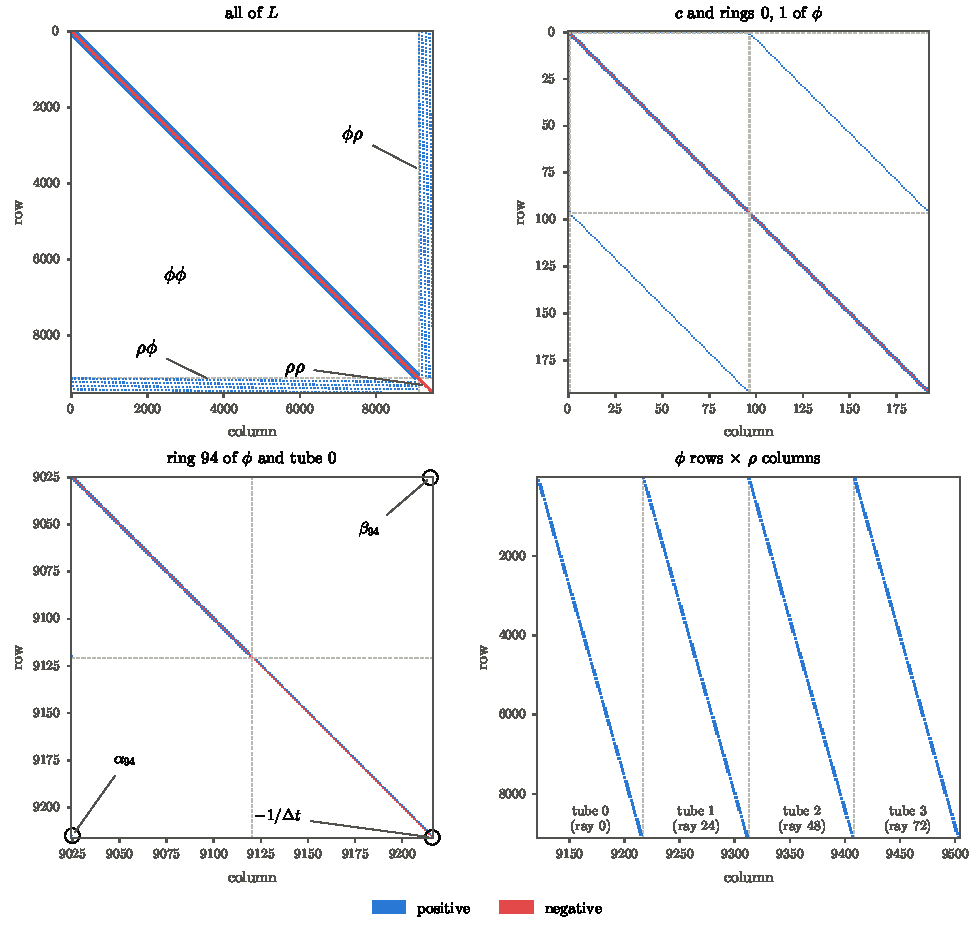
\includegraphics[width=\textwidth]{L_sparsity_96x96.pdf}
\caption{Nonzeros of $L$ at $96 \times 96$, $(a, b) = (1, 1)$: positive in blue, negative (the
diagonal) in red; dashed lines separate blocks. Top left, all $9{,}505$ rows and columns. Top right,
$c$ and rings 0 and 1, one cell per entry: the $c$ row and column, the two ring blocks on the diagonal,
and the radial couplings at $\pm 96$. Bottom left, ring 94 (the last diffusive ring) and tube 0, one cell
per entry: the ring block has no outward coupling, the tube block is upper bidiagonal, the circled
entries are the exchange pair $\beta_{94}, \alpha_{94}$ of ray 0, and the last diagonal entry is the rim
tube cell's $-1/\Delta t$. Bottom right, the $\phi\rho$ block: each tube takes $\beta_m$ from one cell
per ring, on its own ray.}
\label{fig:sparsity}
\end{figure}

\paragraph{Reproducing.} \code{scripts/eigen\_appendix\_L.py} extracts $L$ from the solver,
assembles it from A.1, compares the two, writes the inputs of this appendix and rebuilds the PDF, in
about 30\,s on one CPU. The extraction steps each unit vector with \code{\_Operator.step} of
\code{mass\_analysis\_modal.py}, which calls the same \code{comp\_DL\_AL\_kp1\_2step} and
\code{u\_center} as Section~2.3. The solver files are unchanged between
commit \code{dca5c97}, which this note used, and \code{d417235}, which built this appendix.

\end{document}
